% Präambel
\documentclass[%
fontsize=12pt,					% Schriftgröße
paper=a4,						% Papierformat
twoside=false, 					% einseitiges (oneside) oder zweiseitiges (twoside) Dokument
listof=totoc, 					% Tabellen- und Abbildungsverzeichnis ins Inhaltsverzeichnis
bibliography=totoc,				% Literaturverzeichnis ins Inhaltsverzeichnis aufnehmen
titlepage, 						% Titlepage-Umgebung statt \maketitle
headsepline, 					% horizontale Linie unter Kolumnentitel
%abstracton,					% Überschrift beim Abstract einschalten, Abstract muss dazu in {abstract}-Umgebung stehen
DIV=12,							% Satzspiegeleinstellung, 12 ist Standar bei KOMA
%BCOR=6mm,						% Bindekorrektur, die den Seitenspiegel um 6mm nach rechts verschiebt,
cleardoublepage=empty,			% Stil einer leeren eingefügten Seite bei Kapitelwechsel
parskip,							% Absatzabstand bei Absatzwechsel einfügen
ngerman
]{scrbook}			
\usepackage[setspace=false]{scrhack}
\usepackage[utf8]{inputenc} 	% ermöglicht die direkte Eingabe von Umlauten
\usepackage[T1]{fontenc} 		% Ausgabe aller zeichen in einer T1-Codierung (wichtig für die Ausgabe von Umlauten!)
\usepackage{babel} 	% deutsche Trennungsregeln und Übersetzung der festcodierten Überschriften
\setlength{\parindent}{0ex} 	% bei neuem Abschnitt nicht einrücken
%------
% Folgende Einstellungen entsprechen den Vorgaben der Leitlinien
\usepackage[onehalfspacing]{setspace}
% Ende Leitlinien
%------
%------
% Folgende Einstellungen sind bei größeren Arbeiten mit viel Text zu empfehlen.
% Hierbei oben DIV=16 einstellen und Zeile \usepackage[onehalfspacing]{setspace} auskommentieren.
%\linespread{1.2}\selectfont     % Zeilenabstand erhöhen - größere Werte als 1.2 nicht verwenden!!
% Ende Einstellung große Arbeiten mit viel Text.
%------

\usepackage{siunitx}			% Vereinfachte Eingabe von Einheiten in Formeln
\sisetup{
	number-unit-product = \;,
	inter-unit-product = \:,
	exponent-product = \cdot,
	output-decimal-marker = {,}
}

\usepackage{graphicx}  			% Einbinden von Grafiken erlauben
\usepackage[format=hang,		% Formatierungen von Unter- / Überschriften
font=normal,
labelfont=bf,
justification=RaggedRight,
singlelinecheck=true,
aboveskip=1mm
]{caption}

\usepackage[backend=biber, %% Hilfsprogramm "biber" beim Compilieren nutzen (statt "biblatex" oder "bibtex")
style=alphabetic, %% Zitierstil (siehe Dokumentation)
natbib=true, %% Bereitstellen von natbib-kompatiblen Zitierkommandos
hyperref=true, %% hyperref-Paket verwenden, um Links zu erstellen
]{biblatex}
\setcounter{biburllcpenalty}{7000}
\setcounter{biburlucpenalty}{8000}
\addbibresource{literature/literatur1.bib} %% Einbinden der bib-Datei. Endung .bib unbedingt ergänzen
\addbibresource{literature/literatur2.bib} %% Einbinden mehrerer bib-Dateien mit zusätzlichem \addbibresource - Befehl

\usepackage{csquotes}

% Folgende Zeilen sind auszukommentieren, falls runde Klammern und ein vgl. bei Zitaten erscheinen sollen.
%\makeatletter
%\renewcommand{\@cite}[2]{(vgl. {#1\if@tempswa , #2\fi})} 
%\renewcommand{\@biblabel}[1]{(#1)}
%\makeatother

\usepackage{pdfpages}

\usepackage{enumitem}			% Erlaubt Änderung der Nummerierung in der Umgebung enumerate

\usepackage{amsmath}			% Ergänzungen für Formeln
\usepackage{textcomp} 			% zum Einsatz von Eurozeichen u. a. Symbolen
\usepackage{eurosym}			% bessere Darstellung Euro-Symbol mit \euro

\usepackage[					% Einstellunge Paket hyperref
hyperfootnotes=false,			% im pfd-Output Fußnoten nicht verlinken
hidelinks						% Entfernen von farbigen Umrandungen der Links
]{hyperref}

\usepackage{makeidx}			% Paket zur Erstellung eines Index
\usepackage[intoc]{nomencl} 	% zur Erstellung des Abkürzungsberzeichnisses

\usepackage[					% Einstellungen für Fußnoten
bottom,							% Ausrichtung unten
multiple,						% Trennung durch Seperator bei mehreren Fußnoten
hang,
marginal
]{footmisc}

\usepackage{calc}				% Paket zum Berechnen von Längen z.B. 0.8\linewidth

\usepackage{xcolor} 			% einfache Verwendung von Farben in nahezu allen Farbmodellen

\usepackage{listings}			% Darstellung von Quellcode mit den Umgebungen {lstlisting}, \lstinline und \lstinputlisting
\lstset{literate=				% Damit können Umlaute innerhalb Listings geschrieben werden
	{Ö}{{\"O}}1
	{Ä}{{\"A}}1
	{Ü}{{\"U}}1
	{ß}{{\ss}}1
	{ü}{{\"u}}1
	{ä}{{\"a}}1
	{ö}{{\"o}}1
}
\definecolor{mygreen}{rgb}{0,0.6,0}
\definecolor{mygray}{rgb}{0.5,0.5,0.5}
\definecolor{mymauve}{rgb}{0.58,0,0.82}
\lstset{ %
	backgroundcolor=\color{white},   % choose the background color; you must add \usepackage{color} or \usepackage{xcolor}; should come as last argument
	basicstyle=\footnotesize,        % the size of the fonts that are used for the code
	breakatwhitespace=false,         % sets if automatic breaks should only happen at whitespace
	breaklines=true,                 % sets automatic line breaking
	captionpos=t,                    % sets the caption-position to (b) bottom or (t) top
	commentstyle=\color{mygreen},    % comment style
	deletekeywords={...},            % if you want to delete keywords from the given language
	escapeinside={\%*}{*)},          % if you want to add LaTeX within your code
	escapeinside={(*@}{@*)},
	extendedchars=true,              % lets you use non-ASCII characters; for 8-bits encodings only, does not work with UTF-8
	frame=none,	                   	% "single" adds a frame around the code; "none"
	keepspaces=true,                 % keeps spaces in text, useful for keeping indentation of code (possibly needs columns=flexible)
	keywordstyle=\color{blue},       % keyword style
	language=[LaTeX]TeX,             % the language of the code
	morekeywords={*,nomenclature},   % if you want to add more keywords to the set
	numbers=left,                    % where to put the line-numbers; possible values are (none, left, right)
	numbersep=5pt,                   % how far the line-numbers are from the code
	numberstyle=\tiny\color{mygray}, % the style that is used for the line-numbers
	rulecolor=\color{black},         % if not set, the frame-color may be changed on line-breaks within not-black text (e.g. comments (green here))
	showspaces=false,                % show spaces everywhere adding particular underscores; it overrides 'showstringspaces'
	showstringspaces=false,          % underline spaces within strings only
	showtabs=false,                  % show tabs within strings adding particular underscores
	stepnumber=1,                    % the step between two line-numbers. If it's 1, each line will be numbered
	stringstyle=\color{mymauve},     % string literal style
	tabsize=2,	                   % sets default tabsize to 2 spaces
	title=\lstname                   % show the filename of files included with \lstinputlisting; also try caption instead of title
}

\makeindex						% Indexverzeichnis erstellen
\makenomenclature				% Abkürzungsverzeichnis erstellen

% -----------------------------------------------------------------------------------------------------------------
% Zum Aktualisieren des Abkürzungsverzeichnisses (Nomenklatur) bitte auf der Kommandozeile folgenden Befehl aufrufen :
% makeindex <Dateiname>.nlo -s nomencl.ist -o <Dateiname>.nls
% Oder besser: Kann in TexStudio unter Tools-Benutzer als Shortlink angelegt werden
% Konfiguration unter: Optionen-Erzeugen-Benutzerbefehle: makeindex -s nomencl.ist -t %.nlg -o %.nls %.nlo
% -----------------------------------------------------------------------------------------------------------------

% Hier die persönlichen Daten eingeben:

\newcommand{\titel}{Grundlagen der Metallbearbeitung und Einführung in den Betrieb des Stromnetzes der TWS Netz GmbH}
\newcommand{\untertitel}{}			% ggf. Untertitel mit ergänzenden Hinweisen
\newcommand{\arbeit}{Praxisarbeit T3_1000}
\newcommand{\studiengang}{Elektrotechnik}
\newcommand{\studienrichtung}{Energie- und Umwelttechnik}
\newcommand{\studienschwerpunkt}{}
\newcommand{\autor}{Alexander Dreher}
\newcommand{\matrikelnr}{5642939}
\newcommand{\kurs}{TFE22-1/TEU22}
\newcommand{\firma}{TWS Netz GmbH}
\newcommand{\abgabe}{\today}
\newcommand{\betreuerdhbw}{}			% Gutachter der DHBW (nur bei Bachelorarbeit erforderlich)
\newcommand{\betreuerfirma}{Patricia Schmitz}
\newcommand{\jahr}{2023}			% für Angabe im Copyright-Vermerk der Titelseite

% Folgende Zeilen definieren Abkürzungen, um Befehle schneller eingeben zu können
\newcommand{\ua}{\mbox{u.\,a.\ }}
\newcommand{\zB}{\mbox{z.\,B.\ }}
\newcommand{\bs}{$\backslash$}
\newcommand*\diff{\mathop{}\!\mathrm{d}}	% Differentialzeichen
\newcommand*\Diff[1]{\mathop{}\!\mathrm{d^#1}} % Differentialzeichen höherer Ableitung
\newcommand*\jj{\mathop{}\!\mathrm{j}}	% Komplexe Zahl j

% Folgende Zeilen werden benötigt, um Tikz und PGF-Plot-Grafiken einzubinden
\usepackage{pgfplots}
\usepackage{pgfplotstable}
\pgfplotsset{compat=newest,width=0.6\linewidth}
\usepgfplotslibrary{smithchart}
\usepackage{tikz}						% Tikz sollte nach Listings Pakete geladen werden.
\usetikzlibrary{arrows}

\hyphenation{Schrift-ar-ten}


% -------------------------------------------------------------------------------------------
%                     Beginn des Dokumenteninhalts
% -------------------------------------------------------------------------------------------
\begin{document}
\let\texteuro\euro						% Eingabe \texteuro, € oder \euro erzeugt gleiches Ergebnis
\setcounter{secnumdepth}{3}				% Nummerierungstiefe fürs Inhaltsverzeichnis
\setcounter{tocdepth}{3}
\sffamily								% für die Titelei serifenlose Schrift verwenden

% ------------------------------ Titelei -----------------------------------------------------

\thispagestyle{plain}
\hypersetup{pageanchor=false}
\begin{titlepage}
\enlargethispage{4.0cm}
\sffamily 								% Serifenlose Grundschrift für die Titelseite einstellen

\parbox{0.5\linewidth}{
\begin{flushleft}
	\includegraphics[width=0.5\linewidth]{images/Firmenlogo}\\[5ex]
\end{flushleft}
}
\parbox{0.5\linewidth}{
\begin{flushright}
	
\includegraphics[width=0.5\linewidth]{images/DHBW_d_R_FN_46mm_4c}\\[5ex]
\end{flushright}
}
				

\begin{center}

{\fontsize{20.74pt}{24pt}\selectfont
\textbf{\titel}\\[1.5ex]}
{\fontsize{14pt}{17pt}\selectfont
\textbf{\untertitel}\\[5ex]}
{\fontsize{17pt}{20pt}\selectfont
\textbf{\arbeit}\\[2ex]}
{\fontsize{14pt}{17pt}\selectfont
Studiengang \studiengang\\[2ex]}
{\fontsize{12pt}{14pt}\selectfont
Studienrichtung \studienrichtung\\[1ex]
Duale Hochschule Baden-Württemberg Ravensburg, Campus Friedrichshafen\\[5ex]
von\\[1ex]
\autor\\[15ex]}


\end{center}

\begin{flushleft}
{\fontsize{12pt}{14pt}\selectfont
\begin{tabular}{ll}
Abgabedatum:					& \quad \abgabe \\
Bearbeitungszeitraum:		   		& \quad 01.07.2023 - 31.09.2023   \\ 
Matrikelnummer: 			& \quad \matrikelnr \\ 
Kurs: 							& \quad \kurs \\
Ausbildungsfirma:	 			& \quad \firma \\ 
Betreuer der Ausbildungsfirma:  & \quad \betreuerfirma \\ 
%Gutachter der Dualen Hochschule: & \quad \betreuerdhbw \\ [2ex]
\end{tabular}
}
\end{flushleft}
%%%%% Nachfolgende Zeilen einkommentieren, wenn Copyrightvermerk gewünscht ist
%\begin{flushleft}
%{\fontsize{11pt}{13pt}\selectfont
%Copyrightvermerk:\\
%Dieses Werk einschließlich seiner Teile ist \textbf{urheberrechtlich geschützt}. Jede Verwertung außerhalb der engen Grenzen des Urheberrechtgesetzes ist ohne Zustimmung des Autors unzulässig und strafbar. Das gilt insbesondere für Vervielfältigungen, Übersetzungen, Mikroverfilmungen sowie die Einspeicherung und Verarbeitung in elektronischen Systemen.
%}
%\end{flushleft}
%\begin{flushright}
%{\fontsize{11pt}{13pt}\selectfont \copyright{} \jahr }
%\end{flushright}
\end{titlepage}

\cleardoublepage
\hypersetup{pageanchor=true}
 				% erzeugt die Titelseite
\pagenumbering{roman}					% kleine, römische Seitenzahlen für Titelei
%% Ggf. folgende Zeile auskommentieren, falls der Sperrvermerk gewünscht ist.
%\chapter*{Sperrvermerk} %*-Variante sorgt dafür, das der Sperrvermerk nicht im Inhaltsverzeichnis auftaucht
%gemäß Ziffer 1.1.13 der Anlage 1 zu §§ 3, 4 und 5  der Studien- und Prüfungsordnung für die Bachelorstudiengänge im Studienbereich Technik der Dualen Hochschule Baden-Württemberg vom 29.09.2017 in der Fassung vom 25.07.2018:
%
%Der Inhalt dieser Arbeit darf weder als Ganzes noch in Auszügen Personen außerhalb des Prüfungsprozesses und des Evaluationsverfahrens zugänglich gemacht werden, sofern keine anders lautende Genehmigung vom Dualen Partner vorliegt.
%
%Musterstadt, den \today \\[4ex]
%
%\rule[-0.2cm]{5cm}{0.5pt} \\
%
%\textsc{\autor} \\[10ex]

\chapter*{Erklärung} %*-Variante sorgt dafür, dass die Erklärung nicht im Inhaltsverzeichnis auftaucht

gemäß Ziffer 1.1.13 der Anlage 1 zu §§ 3, 4 und 5  der Studien- und Prüfungsordnung für die Bachelorstudiengänge im Studienbereich Technik der Dualen Hochschule Baden-Württemberg vom 29.09.2017 in der Fassung vom 10.07.2023.

Ich versichere hiermit, dass ich meine Bachelorarbeit (bzw. Projektarbeit oder Studienarbeit bzw. Hausarbeit) mit dem Thema:

\begin{quote}
	\textit{\titel} %-\textit{ \untertitel }
\end{quote}

selbstständig verfasst und keine anderen als die angegebenen Quellen und Hilfsmittel benutzt habe. Ich versichere zudem, dass die eingereichte elektronische Fassung mit der gedruckten Fassung übereinstimmt.\\[6ex]

Ravensburg, den \today \\[1ex]

\rule[-0.2cm]{5cm}{0.5pt} \\

\autor %\\[10ex]

\rmfamily

%\thispagestyle{empty}

%\clearpage 				% Einbinden der eidestattlichen Erklärung
\chapter*{Kurzfassung} %*-Variante sorgt dafür, das Abstract nicht im Inhaltsverzeichnis auftaucht

Hier kommt eine Kurzfassung hin

\cleardoublepage
   			% Einbinden des Abstracts

\tableofcontents						% Erzeugen des Inhalsverzeichnisses
\cleardoublepage

% --------------------------------------------------------------------------------------------
%                    Inhalt der Bachelorarbeit
%---------------------------------------------------------------------------------------------
\pagenumbering{arabic}					% arabische Seitenzahlen für den Hauptteil

\rmfamily

\chapter{Einleitung}
\label{cha:Einleitung}

... Text Einleitung ...

Am Ende der Einleitung: Die Arbeit ist wie folgt gegliedert: ... 
\chapter{Grundlagen}
\label{cha:Grundlagen}

... Theoretische Grundlagen (vielleicht auch zitiert aus Standardwerken, wie z.B. aus \autocite{Tipler.2019}), Rechercheergebnisse, Stand der Technik \index{Stand der Technik} (ggf. zitiert aus Hochschulschriften, welche Online verfügbar sind, wie z.B.~\autocite{Ziegler.2017}), etc.
\chapter{Konzeptentwurf}
\label{cha:Konzeptentwurf}

... Text Konzeptentwurf: Gegenüberstellung verschiedener Lösungsansätze und Lösungsgenerierung, etc.
\chapter{Umsetzung}
\label{cha:Umsetzung}

... Text Umsetzung: Beschreibung der Umsetzung und eigener Untersuchungen ...
\chapter{Verifikation und Diskussion}
\label{cha:Verifikation}

... Verifikation, Auswertung, Lösungsbewertung, Diskussion der Ergebnisse
\chapter{Zusammenfassung}
\label{cha:zusammenfassung}

Die Projektarbeit befasste sich mit den Strukturen und Tätigkeiten des Elektrikers für Betriebstechnik in der TWS Netz GmbH. Dazu wurden verschiedenste 
Tätigkeitsschwerpunkte genannt, welche eine große Rolle im Alltag dieses Berufes spielen. Sie dienen nicht nur als Hilfsstellung für jegliche Probleme
im Stromnetz, sondern besitzen zudem eine fördernde Wirkung für eine theoretische, als auch praktische Annahme und Lösung eines Problems. Dazu wurden 
Fertigkeiten im Bereich der Metallbearbeitung geschult, welche das Verständnis für die richtige Wahl des Werkzeuges und dem richtigen Verfahren förderten. 
Diese Entscheidung spielt eine wichtige Rolle in der Lösung von individuellen Problemstellungen, da Sie am Anfang eines Problems getroffen wurde und 
verantwortlich für eine nachhaltige und zielorientierte Lösung ist. Bei einer nicht idealen Entscheidung, kann es zu zeit-, kosten- oder umwelttechnischen 
Konsequenzen kommen, welche das Image des Unternehmens schädigen und zusätzlich ein Misstrauen beim Kunden verursachen. Um solche Entscheidungen genauer 
zu kalkulieren wurden Kenntnisse zur Berechnung mathematischer Theoreme im Bereich Elektrotechnik gefördert. Diese theoretischen Grundlagen wurden angewandt, 
um die praktischen Vorgehensweisen anhand mathematischer Theoreme zu belegen. Dazu zählen überwiegend die Berechnung von Stromkreisen, Leitungswiderständen 
und Trafoleistungen. Diese Kennwerte tragen zu einem stabilen und zuverlässigen Stromnetz bei und dienen zusätzlich als Grundlage zur Planung neuer 
Umspannstationen oder Schaltfelder. Somit wird nachhaltig für eine Versorgungssicherheit im Netzgebiet der TWS Netz GmbH gesorgt. Es reicht allerdings 
nicht aus, das Stromnetz auf Grundlage von theoretischen Kennwerten zu managen, da die Einflüsse der Umwelt ebenso große Anteile tragen und beseitigt 
werden müssen. Es ist zwar möglich eine ungefähre Lebensdauer \zB eines Holzmasten zu berechnen, allerdings hat die Praxis bewiesen, dass durch äußere 
Einflüsse, diese auch stark abweichen kann. Daher ist es ebenso wichtig das Stromnetz regelmäßig zu kontrollieren, um Abweichungen frühestmöglich zu 
erkennen. Bei Freileitungen können Probleme dieser Art schnell identifiziert und behoben werden, ganz im Gegenteil zu Erdkabeln. Bei diesen müssen 
Strukturen zur ordnungsgemäßen Montage und zur Sauberhaltung der Anlagen eingehalten werden, um dem Kunden ein störungsfreies Netz zu gewährleisten. 
Wichtig sind diese Strukturen vor allem bei Schwachpunkten im Netz, wie \zB den Kabelmuffen. Diese sind besonders anfällig für Netzstörungen, wenn bei 
der Montage nicht auf Genauigkeit geachtet wird. Zudem kann es in diesem Tätigkeitsbereich schnell zur Schädigung der Umwelt kommen, wenn das Erdreich 
durch austretendes Öl von alten Kabeln belastet wird. Des Weiteren ist es wichtig Richtlinien und Sicherheitsvorschriften, vor allem im Bereich der 
Mittelspannung einzuhalten, da es in diesem Bereich schnell zu Personenschäden kommt und die Umwelt stark belastet werden kann. Genannte Beispiele sind 
unter Spannung stehende Kabel oder \ce{SF_6} Schaltanlagen. Ziel ist stets ein stabiles und leistungsfähiges Netz gegenüber dem Kunden zu garantieren. Hierzu 
trägt ein Ring- oder Maschennetz positiv bei und sorgt somit im Nieder-, als auch Mittelspannungsbereich für eine flexible und krisensichere Versorgung. 
All diese Tätigkeiten und Strukturen der TWS Netz GmbH sorgen für eine Verknüpfung der theoretischen Kenntnisse mit praktischen Problemstellungen und 
fördern eine eigenständige Lösung eines Problems unter Anwendung ingenieurstechnischer Vorgehensweisen.
\chapter{Vorlagen}
\label{cha:Vorlagen}

\section{Standards}
\subsection{Listenumgebungen und Fußnoten}
Jede wissenschaftliche Arbeit ist natürlich auf Fußnoten\footnote{das sind die kleinen zusätzlichen Hinweise am unteren Rand der Seite} angewiesen. Zudem kommt es immer wieder vor, dass man \marginpar{Bemerkung!}
\begin{itemize}
\item[-] Aufzählungen
\item[+] Nummerierungen oder
\item[*] Definitionen 
\end{itemize}
verwenden muss. In einer Aufzählung \footnote{also in einer \textit{enumerate}-Umgebung} würde das dann so aussehen.
\begin{enumerate}
\item Aufzählungen
\item Nummerierungen oder
\item Definitionen 
\end{enumerate}

In einer Definition \footnote{also in einer \textit{description}-Umgebung} sähe das dann wohl eher so aus:

\begin{description}
\item[Silvester] Jahresendfeier mit Feuerwerk und Alkoholgenuss
\item[Böller] Feuerwerkszubehör ohne visuellen Reiz, dafür aber recht laut
\end{description}

\subsection{Verweise und Zitate}

Bilder, Tabellen und sonstige ins Dokument eingebundene Objekte müssen im Text ausführlich beschrieben und diskutiert werden. Um eine Verbindung zwischen Text und beschriebenes Objekt herzustellen, können Referenzen hergestellt werden. Auch zu anderen Textstellen können Referenzen eingebaut werden, \zB eine Referenz auf das Kapitel \ref{cha:wortberge} auf Seite \pageref{cha:wortberge}. Dazu muss das referenzierte Objekt (hier das entsprechende Kapitel) zuvor entsprechend mit dem Befehl \textit{\bs \textcolor{blue}{label}\{Labelbezeichner\}} versehen worden sein. Bei der Angabe des Labelbezeichners bietet es sich zur besseren Übersichtlichkeit an, im Label zu benennen, um welche Referenz es sich handelt (cha: für Kapitelüberschrift, sec: für die Abschnittsüberschrift, fig: für Bildunterschriften, tab: für Tabellenüberschriften, eqn: für Gleichungen, lst: für Listings, etc.).

Wesentlicher Bestandteil einer wissenschaftlichen Arbeit ist die Angabe der verarbeiteten Literaturangaben. In \cite[S. 3]{Vo.2013} sind einige Möglichkeiten zur Zitierweise von Literaturangaben aufgeführt. Sie können aber einfach die in diesem Absatz verwendete Möglichkeiten nutzen, entweder mit Angabe einer Seitenzahl, wie in Listing~\ref{lst:cite} in Zeile~\ref{lst:cite:mitSeite} oder ohne Angabe einer Seitenzahl, wie in Zeile~\ref{lst:cite:ohneSeite} dargestellt ist.

%\caption{Ein Listing}
\label{lst:cite}
\begin{lstlisting}[caption=LaTeX-Befehle zur Angabe von Literaturangaben,label=lst:cite]
\cite[S. 3]{Vo.2013}	% mit Angabe einer Seitenzahl (*@\label{lst:cite:mitSeite}@*)
\cite{Vo.2013}	% einfachste und meist völlig ausreichende Methode (*@\label{lst:cite:ohneSeite}@*)
\end{lstlisting}

\subsection{Indexe und Verzeichnisse}
Eine der großen Stärken von LaTeX ist die relativ bequeme Erstellung mehrerer Verzeichnisse. Verzeichnisse helfen, das Dokument übersichtlich zu gestalten und schnell bestimmte Stellen im Dokument wiederzufinden. Diese Vorlage erstellt neben dem Inhalts-, Abbildungs- und Tabellenverzeichnis auch ein Indexverzeichnis und ein Abkürzungsverzeichnis. Eine weitere Option ist die Erstellung eines Glossars, auf diese Funktion wird hier aber nicht weiter eingegangen.

Einen Eintrag in das Abkürzungsverzeichnis lässt sich über den nachfolgenden Befehl erreichen. Das entsprechende Beispiel ist im Quelltext an dieser Stelle zu finden.
\begin{lstlisting}
\nomenclature{SI}{Systeme International. 1960 hat ein internationales Komitee die Standardmaßeinheiten (SI-Einheiten) aufgestellt}
\end{lstlisting}

\nomenclature{SI}{Système International. 1960 hat ein internationales Komitee die Standardmaßeinheiten (SI-Einheiten) aufgestellt} % Dieser Befehl erstellt im Abkürzungsverzeichnis einen entsprechenden Eintrag

Allgemeine Abkürzungen werden vorzugsweise in der Datei \glqq \textit{abkuerzungen.tex}\grqq ~gesammelt. Es bietet sich an, auch verwendete Formelzeichen in das Abkürzungsverzeichnis zu setzen. Dabei ist zu beachten, dass Formelzeichen grundsätzlich kursiv gestellt sein müssen, d.h. dass diese im Mathematikmodus gesetzt sind. Ein Beispiel zum Formelzeichen für die Zeit $t$ \nomenclature{$t$}{Zeit} sei hier gegeben.

Einen Eintrag in das Indexverzeichnis, bzw. Sachwortverzeichnis erreicht man über folgenden Befehl:\\
\textit{\textbackslash index \textnormal{\{Indexeintrag\}}}.

Als Beispiel soll hier das Wort Soziologie\index{Soziologie} einen Eintrag im Indexverzeichnis erhalten. Auch Gruppierungen sind hier möglich, z.B. kann man im Index verschiedenes Obst in einem Eintrag nennen, also z.B. den Apfel\index{Obst!Apfel} oder die Birne\index{Obst!Birne}.

% --------------------------------------------------------------------------------------------------------------------------

\section{Verschiedene Umgebungen}
\label{sec:Umgebungen}

\subsection{Einsatz von Gleitumgebungen}

Gleitumgebungen werden für Grafiken, Bilder und Tabellen verwendet. Beim Übersetzen des Dokuments sucht Latex die optimale Position des Gleitobjekts. Die Algorithmus kann durch die Optionen [hbt]~(Abkürzung für \textbf{h}ere, \textbf{b}ottom, \textbf{t}op) beeinflusst werden. In den folgenden Abschnitten werden die unterschiedlichen Gleitumgebungen vorgestellt.

\subsection{Tabellen}

%Tabellen selbst werden in der Umgebung \textit{tabular} oder \textit{tabularx}gesetzt. Um die Tabelle zu einem Gleitobjekt zu machen, muss diese dann in die Umgebung \textit{table} gesetzt werden. Tabellen erhalten im Gegensatz zu Grafiken eine \glqq Überschrift\grqq, keine \glqq Unterschrift\grqq.
%
%\begin{table}[hbt]
%\captionabove{Beispiel für eine Tabelle} 
%\centering
%\begin{tabular}{c|c|c}
%\hline Diese & Tabelle & ist \\ 
%\hline zentriert & und  & verwendet \\ 
%\hline vertikale & Trennzeichen &  .\\ 
%\hline 
%\end{tabular}
%
%\end{table}

Tabellen, wie z.B. die Tabelle~\ref{tab:tabbsp} werden mit dem Befehl \textit{tabular} definiert und in die Gleitumgebung \textit{table} eingebunden. Im Gegensatz zu Grafiken, in welche mit einer Bildunterschrift versehen sind, besitzen Tabellen eine Überschrift.

\begin{table}[hbt]
	\caption{Tabelle mit wenig sinnvollem Inhalt und ein paar Linien.}
	\centering
	\begin{tabular}{|cc|c p{0.3\linewidth}} % vertikale Linien werden mit | festgelegt, Tip: Tabellen sind ohne vertikale Linien schöner. Das c bedeutet zentriert. Die Spaltenbreite richtet sich dann nach dem Inhalt.
		\textbf{Sp. 1 }& \textbf{Sp. 2} & \textbf{Sp. 3} &\textbf{Noch \grq ne Spalte mit fester Breite, womit ein Zeilenumbruch, oder mehrere erzeugt werden}\\
		\hline 
		\hline 
		Was & auch & immer & \\ 
		\hline 
		Sie & schreiben & möchten. &\\ 
		\hline 
	\end{tabular} 
	\label{tab:tabbsp}
\end{table}



\subsection{Einbindung von Bildern}

Bilder, Grafiken und Diagramme bereichern eine wissenschaftliche Arbeit und dienen dazu, bestimmte Sachverhalte zu veranschaulichen. Meist wird in \LaTeX~ein Bild als jpg- oder pdf-Datei mit dem Befehl \textit{includegraphics} eingebunden (siehe Bild~\ref{fig:matlab}). Mit einem anderen Programm muss diese Datei also zuerst erstellt werden. Die meisten Grafikprogramme können jpg-Dateien exportieren. Das jpg-Format hat aber den Nachteil, dass sämtliche Inhalte komprimiert werden, auch Linien und in das Bild eingebettete Schriftzüge. Oft ist die Komprimierung so stark, dass Kompressionsartefakte zu erkennen sind. Das pdf-Format hat den Vorteil, dass es Grafiken vektorbasiert speichern kann. Vektorgrafiken sind bei beliebiger Vergrößerung pixelgenau und zeigen keine Unschärfen. Die Qualität einer pdf-Grafik ist natürlich nur dann gut, wenn bei der Erstellung in der gesamten Kette Daten vektorbasiert gespeichert wurden. Es hilft also nicht, eine jpg-Datei mit schlechter Qualität in eine pdf-Datei zu wandeln.

Bei der Erstellung von Grafiken mit eingebetteten Schriftzügen ist darauf zu achten, dass die Schriftart und Schriftgröße der verwendeten Schriftart und -größe des umgebenden Textes entspricht. Diese Anforderung ist aber meist schwer zu erfüllen, da die meisten Grafik-Programme keine \LaTeX-Schriftarten anbieten und oft unklar ist, welche Schriftart und -größe bei der Finalisierung der Arbeit verwendet wird.

Ein Bild wird in eine sogenannte Gleitumgebung \textit{figure} gesetzt. \LaTeX~entscheidet bei einer Gleitumgebung selbst, an welcher Stelle im Dokument das Bild platziert wird. Mit den optionalen Parametern \textit{hbt} lässt sich die Präferenz für die Positionierung auf der Seite angeben (\textit{h}ere, \textit{b}ottom \textit{t}op).

Bild~\ref{fig:matlab} zeigt ein Beispiel für eine nicht optimal gestaltete Grafik: Durch die starke Komprimierung werden Artefakte sichtbar, die Schriftgröße ist zu klein und kann nicht genau entziffert werden. Das Bild ist über einen Screenshot einer Matlab-Grafik erstellt worden.


Eine Lösung dieses Problems ist die Erstellung von Grafiken und Diagrammen mit speziellen Programmen, die wie \LaTeX, nicht nach dem WYSIWYG-Prinzip\footnote{What you see is what you get.} arbeiten. Der Vorteil dieses Vorgehens ist, dass erst bei der Erstellung des \LaTeX-Dokuments die Schrift in die Grafik entsprechend der Dokumentvorgaben für Schriftart und -größe eingebettet wird.

In den folgenden Abschnitten werden Beispiele für Diagramme und Grafiken gegeben, die wie in \LaTeX~mit entsprechenden Kommandos programmiert werden.

\subsection{Erstellen von Diagrammen}

Wenn Sie Funktionen oder Messwerte darstellen möchten, empfehle ich Ihnen die Verwendung des \LaTeX-Packages \textit{pgfplot}. Auch hier wird das Diagramm in die Gleitumgebung \textit{figure} eingebettet. Das Diagramm selbst wird in einer separaten .tex-Datei programmiert und mit dem Befehl \textit{input} in das Hauptdokument geladen. \textit{pgfplot} benutzt zur Darstellung der grafischen Elemente die Umgebung \textit{tikzpicture}. Ein Beispiel ist in Bild~\ref{fig:pgfplot} zu sehen.

\begin{figure}[hbt]
	\centering
	\begin{tikzpicture}
		\begin{axis}[scale=1.3,legend entries={Messwerte mit Fehlerbalken,
			$\pgfmathprintnumber{\pgfplotstableregressiona} \cdot x  
			\pgfmathprintnumber[print sign]{\pgfplotstableregressionb}$}, legend style={draw=none},legend style={at={(0.01,0.98)},anchor=north west},xlabel=Stromstärke $I \; \mathrm{ \lbrack mA \rbrack}$,ylabel=Spannung $U \; \mathrm{ \lbrack V \rbrack}$]
		\addlegendimage{mark=*,blue}
		\addlegendimage{no markers,red}
\addplot+[error bars/.cd, y dir=both,y explicit]
table[x=x,y=y,y error=errory] 
{pgfplot/messdaten_mitfehler.dat};
\addplot table[mark=none,y={create col/linear regression={y=y}}]
{pgfplot/messdaten_mitfehler.dat};
	\end{axis}
\end{tikzpicture}
	\caption[Diagramm, mit dem \textit{pgfplot}-Befehlssatz]{Ein Diagramm, erstellt in der \textit{tikzpicture}-Umgebung mit dem \textit{pgfplot}-Befehlssatz. Das Diagramm stellt Messdaten, deren Fehlerbalken und eine Regressionskurve dar. Die Messdaten werden von einer separaten Datei eingelesen und die Regressionskurve wurde mit \textit{pgfplot} berechnet und erstellt.}
	\label{fig:pgfplot}
\end{figure}

Im Internet finden Sie eine Vielzahl an weiteren Beispielen. \textit{pgfplot} bietet nahezu jeden denkbaren Diagrammtyp an, auch spezielle Diagramme, wie z.B. ein Smith-Diagramm (siehe Abbildung~\ref{fig:smith}), was in der Hochfrequenztechnik oft verwendet wird und mit Programmen wie EXCEL nicht erstellt werden kann.

\begin{figure}[hbt]
	\centering
	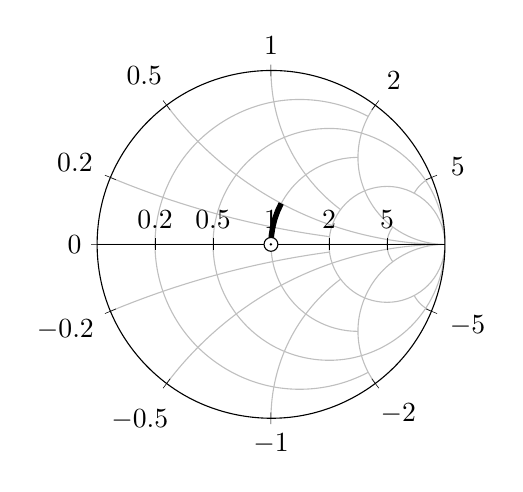
\begin{tikzpicture}
	\begin{smithchart}[
	show origin,
	width=6cm,
	]
	\addplot[mark=none,line width=2]
	coordinates{
		(1, 0) (1, 0.1) (1,0.2) (1,0.3) (1,0.4) (1,0.5) (1,0.5)
	};
	\addplot[mark=none,line width=0.5]
	coordinates{
		(1, 0) (-0.3, 0)  % this one is not drawn outside!!!
	};
	\end{smithchart}
	\end{tikzpicture}
\caption[Smith-Diagramm]{Smith-Diagramm}
\label{fig:smith}
\end{figure}

Ein weiteres Beispiel eines Diagramms ist in Bild~\ref{fig:historamm} dargestellt. Neben der Darstellung eines Histogramms von Messdaten ist eine Gaussfunktion als Näherung angegeben. Eine Erarbeitung eines entsprechenden Diagramms mit EXCEL ist nicht weniger aufwändig und die hier beschriebene Vorgehensweise hat den Vorteil, dass sämtliche Parameter (Achsenbeschriftung, Legende, Farben, Symbole, Beschriftungen) direkt im \LaTeX-Editor vorgenommen werden können.

\begin{figure}[hbt]
	\centering
	\input{pgfplot/mess5s_histogramm.tex}
	\caption[Histogramm der Häufigkeitsverteilung für eine Zeitmessung]{Histogramm der Häufigkeitsverteilung für die Zeitmessung. Der grau markierte Bereich gibt das Vertrauensintervall für $1 \cdot \sigma $ an.}
	\label{fig:historamm}
\end{figure}

Sollte \textit{pgfplot} trotzdem zu aufwändig erscheinen, so sei das Programm Origin als weitere Empfehlung gegeben. Origin hat einen mächtigen Funktionsumfang, bietet sich gut an, um viele Messdaten zu verwalten und kann auch EXCEL-Dateien einbinden. Das Programm Origin ist als Studentenversion für ca. 100 EUR verfügbar. Die DHBW in Friedrichshafen hat ein paar wenige Netzwerklizenzen. Wenden Sie sich gerne an Hr. Prof. Kibler, sofern Sie Interesse haben.


\begin{figure}[hbt]
	\centering
	\includegraphics[width=0.7\linewidth]{origin/mess_fehlerbalken_origin}
	\caption{Diagramm erstellt mit Origin}
	\label{fig:origin}
\end{figure}

Mit vielen anderen Programmen lassen sich Diagramme darstellen, orientieren Sie das Erscheinungsbild Ihres Diagramms an den hier gegebenen Beispielen.

%\includegraphics[width=1.4in,height=1.5in,clip,keepaspectratio]{1336385206-131-kibler}}]

% needed in second column of first page if using \IEEEpubid
%\IEEEpubidadjcol

\subsection{Erstellen von Grafiken}

Zur Erstellung von Grafiken kann man im einfachsten Fall PowerPoint benutzen. Mit einem rechten Mausklick auf ein grafisches Element lässt sich dieses als emf-Datei exportieren (emf-Dateien speichern Grafiken vektorbasiert ab). Die emf-Datei kann dann z.B. mit XnView leicht in das pdf-Format übersetzt werden. Mit einem Mac können Sie Grafiken aus PowerPoint direkt im pdf-Format exportieren. Problematisch ist, wie oben schon beschrieben, die Auswahl einer geeigneten Schriftart in der PowerPoint-Grafik.

In \LaTeX~können alternativ grafische Elemente direkt in der Kommandozeile angegeben werden. Hierfür gibt es diverse Packages, z.B. \textit{tikzpicture}. Die Einbindung einer solchen Grafik ist analog zur Vorgehensweise bei einem \textit{pgfplot}-Diagramm. Zur Erstellung einer  \textit{tikzpicture}-Grafik kann das Hilfsprogramm TikzEdt verwendet werden.

\begin{figure}[hbt]
	\centering
	%\includegraphics[width=0.3\linewidth]{bilder/le_block_p}
	\input{tikz/le_block_tt.tex}
	\caption[Tikzpicture Grafik]{Tikzpicture-Grafik, erstellt mit TikZ.}
	% Die Angabe in der eckigen Klammer würde für den Eintrag in einem Abbildungsverzeichnis verwendet werden. Manche Angaben in der Bildunterschrift sind im verzeichnis ggf. nicht erforderlich.
	\label{fig:le_block_p}
\end{figure}

\subsection{Einsatz von Programmlistings}
Für die Vorlage wird das paket \textit{listings} verwendet. Für die geeignete Markierung von Befehlen kann die verwendete Programmiersprache angegeben werden.

\begin{lstlisting}[language=PHP]
define('PATH_site', dirname(PATH_thisScript).'/');
\begin{lstlisting}
if (@is_dir(PATH_site.'typo3/sysext/cms/tslib/')) {
define('PATH_tslib', PATH_site.'typo3/sysext/cms/tslib/');
} elseif (@is_dir(PATH_site.'tslib/')) {
define('PATH_tslib', PATH_site.'tslib/');
} else {
}
\end{lstlisting}

Das Paket \textit{listings} bietet zahlreiche Konfigurationsmöglichkeiten, um die Quellcodedarstellung an die eigenen Wünsche anzupassen. In einer fertig konfigurierten TexLive-Umgebung erfahren Sie mit dem Kommando

\begin{verbatim}
user@client:~> texdoc listings
\end{verbatim}				% Verbatim ist eine einfache Alternative zu lstlistings und erlaubt auf einfache Weise die abgesetzte Darstellung von Code.

mehr über die Möglichkeiten des Pakets.


\subsection{Formeln}
\label{sec:formeln}

Formeln lassen sich in \LaTeX~ganz einfach schreiben, wie bereits zu Beginn der Arbeit auf Seite~\pageref{cha:Einleitung} erwähnt wurde. Es gibt unterschiedliche Umgebungen zum Schreiben von Formeln. Z.B. direkt im Text $v=s/t$ oder abgesetzt

\[F=m \cdot a\]

oder auch, wie in wissenschaftlichen Dokumenten üblich, nummeriert

\begin{equation}
P=\frac{U^2}{R} \quad .
\label{eqn:leistung}
\end{equation}

Mit einem Label in Formel~\ref{eqn:leistung} lassen sich natürlich auch Formeln im Text referenzieren. \LaTeX~verwendet im Formelmodus einen eigenen Schriftsatz, welcher entsprechend der gängigen Konventionen kursive Zeichen verwendet. Sollen im Formelmodus Einheiten in normaler Schriftart eingefügt werden, dann kann dies über den Befehl \textit{\textbackslash mathrm}\{\} erwirkt werden, wie im Quellcode von Formel~\ref{eqn:leistungMitEinh} zu sehen ist.

\begin{equation}
P=\frac{U^2}{R} = \frac{\left( 100~\mathrm{V}\right)^2}{100~\Omega} = 100~\mathrm{W}\quad .
\label{eqn:leistungMitEinh}
\end{equation}

Zum direkten Vergleich sind die Einheiten in Formel~\ref{eqn:leistungMitEinhfalsch} falsch dargestellt:

\begin{equation}
P=\frac{U^2}{R} = \frac{\left( 100~V\right)^2}{100~\Omega} = 100~W
\label{eqn:leistungMitEinhfalsch}
\end{equation}

Das sind nur ein paar wenige Beispiele und es gibt sehr viele Packages, um Besonderheiten in Formeln realisieren zu können. Nennen Sie Formeln nur, wenn diese zum besseren Verständnis auch wirklich nützlich sind.

Nachfolgend sind ein paar beliebig gewählte Beispiele zu mathematischen Ausdrücken aufgeführt:

\subsubsection{Arrays}

Arrays of mathematics are typeset using one of the matrix environments as 
in
\[
\begin{bmatrix}
1 & x & 0 \\
0 & 1 & -1
\end{bmatrix}\begin{bmatrix}
1  \\
y  \\
1
\end{bmatrix}
=\begin{bmatrix}
1+xy  \\
y-1
\end{bmatrix}.
\]
Case statements use cases:
\[
|x|=\begin{cases}
x, & \text{if }x\geq 0\,,  \\
-x, & \text{if }x< 0\,.
\end{cases}
\]
Many arrays have lots of dots all over the place as in
\[
\begin{matrix}
-2 & 1 & 0 & 0 & \cdots & 0  \\
1 & -2 & 1 & 0 & \cdots & 0  \\
0 & 1 & -2 & 1 & \cdots & 0  \\
0 & 0 & 1 & -2 & \ddots & \vdots \\
\vdots & \vdots & \vdots & \ddots & \ddots & 1  \\
0 & 0 & 0 & \cdots & 1 & -2
\end{matrix}
\]

\subsubsection{Delimiters}

See how the delimiters are of reasonable size in these examples
\[
\left(a+b\right)\left[1-\frac{b}{a+b}\right]=a\,,
\]
\[
\sqrt{|xy|}\leq\left|\frac{x+y}{2}\right|,
\]
even when there is no matching delimiter
\[
\int_a^bu\frac{d^2v}{dx^2}\,dx
=\left.u\frac{dv}{dx}\right|_a^b
-\int_a^b\frac{du}{dx}\frac{dv}{dx}\,dx.
\]






\subsubsection{Spacing}

Differentials often need a bit of help with their spacing as in
\[
\iint xy^2\,dx\,dy 
=\frac{1}{6}x^2y^3,
\]
whereas vector problems often lead to statements such as
\[
u=\frac{-y}{x^2+y^2}\,,\quad
v=\frac{x}{x^2+y^2}\,,\quad\text{and}\quad
w=0\,.
\]
Occasionally one gets horrible line breaks when using a list in mathematics such as listing the first twelve primes  \(2,3,5,7,11,13,17,19,23,29,31,37\)\,.
In such cases, perhaps include \verb|\mathcode`\,="213B| inside the inline maths environment so that the list breaks: \(\mathcode`\,="213B 2,3,5,7,11,13,17,19,23,29,31,37\)\,.
Be discerning about when to do this as the spacing is different.




\subsubsection{Equation arrays}

In the flow of a fluid film we may report
\begin{eqnarray}
u_\alpha & = & \epsilon^2 \kappa_{xxx} 
\left( y-\frac{1}{2}y^2 \right),
\label{equ}  \\
v & = & \epsilon^3 \kappa_{xxx} y\,,
\label{eqv}  \\
p & = & \epsilon \kappa_{xx}\,.
\label{eqp}
\end{eqnarray}
Alternatively, the curl of a vector field $(u,v,w)$ may be written 
with only one equation number:
\begin{eqnarray}
\omega_1 & = &
\frac{\partial w}{\partial y}-\frac{\partial v}{\partial z}\,,
\nonumber  \\
\omega_2 & = & 
\frac{\partial u}{\partial z}-\frac{\partial w}{\partial x}\,,
\label{eqcurl}  \\
\omega_3 & = & 
\frac{\partial v}{\partial x}-\frac{\partial u}{\partial y}\,.
\nonumber
\end{eqnarray}
Whereas a derivation may look like
\begin{eqnarray*}
	(p\wedge q)\vee(p\wedge\neg q) & = & p\wedge(q\vee\neg q)
	\quad\text{by distributive law}  \\
	& = & p\wedge T \quad\text{by excluded middle}  \\
	& = & p \quad\text{by identity}
\end{eqnarray*}

\subsubsection{Functions}

Observe that trigonometric and other elementary functions are typeset 
properly, even to the extent of providing a thin space if followed by 
a single letter argument:
\[
\exp(i\theta)=\cos\theta +i\sin\theta\,,\quad
\sinh(\log x)=\frac{1}{2}\left( x-\frac{1}{x} \right).
\]
With sub- and super-scripts placed properly on more complicated 
functions,
\[
\lim_{q\to\infty}\|f(x)\|_q 
=\max_{x}|f(x)|,
\]
and large operators, such as integrals and
\begin{eqnarray*}
	e^x & = & \sum_{n=0}^\infty \frac{x^n}{n!}
	\quad\text{where }n!=\prod_{i=1}^n i\,,  \\
	\overline{U_\alpha} & = & \bigcap_\alpha U_\alpha\,.
\end{eqnarray*}
In inline mathematics the scripts are correctly placed to the side in 
order to conserve vertical space, as in
\(
1/(1-x)=\sum_{n=0}^\infty x^n.
\)






\subsubsection{Accents}

Mathematical accents are performed by a short command with one 
argument, such as
\[
\tilde f(\omega)=\frac{1}{2\pi}
\int_{-\infty}^\infty f(x)e^{-i\omega x}\,dx\,,
\]
or
\[
\dot{\vec \omega}=\vec r\times\vec I\,.
\]





\subsubsection{Command definition}

\newcommand{\Ai}{\operatorname{Ai}} 
The Airy function, $\Ai(x)$, may be incorrectly defined as this 
integral
\[
\Ai(x)=\int\exp(s^3+isx)\,ds\,.
\]

\newcommand{\D}[2]{\frac{\partial #2}{\partial #1}}
\newcommand{\DD}[2]{\frac{\partial^2 #2}{\partial #1^2}}
\renewcommand{\vec}[1]{\text{\boldmath$#1$}}

This vector identity serves nicely to illustrate two of the new 
commands:
\[
\vec\nabla\times\vec q
=\vec i\left(\D yw-\D zv\right)
+\vec j\left(\D zu-\D xw\right)
+\vec k\left(\D xv-\D yu\right).
\]




\subsubsection{Theorems et al.}

\newtheorem{theorem}{Theorem}
\newtheorem{corollary}[theorem]{Corollary}
\newtheorem{lemma}[theorem]{Lemma}
\newtheorem{definition}[theorem]{Definition}

\begin{definition}[right-angled triangles] \label{def:tri}
	A \emph{right-angled triangle} is a triangle whose sides of length~\(a\), \(b\) and~\(c\), in some permutation of order, satisfies \(a^2+b^2=c^2\).
\end{definition}

\begin{lemma} 
	The triangle with sides of length~\(3\), \(4\) and~\(5\) is right-angled.
\end{lemma}

This lemma follows from the Definition~\ref{def:tri} as \(3^2+4^2=9+16=25=5^2\).

\begin{theorem}[Pythagorean triplets] \label{thm:py}
	Triangles with sides of length \(a=p^2-q^2\), \(b=2pq\) and \(c=p^2+q^2\) are right-angled triangles.
\end{theorem}

Prove this Theorem~\ref{thm:py} by the algebra \(a^2+b^2 =(p^2-q^2)^2+(2pq)^2
=p^4-2p^2q^2+q^4+4p^2q^2
=p^4+2p^2q^2+q^4
=(p^2+q^2)^2 =c^2\).






% ---- Literaturverzeichnis ----------
\interlinepenalty 10000					% Verhindert einen Umbruch mitten in Literatureinträgen
\printbibliography						% Erstellen des Literaturverzeichnisses

% -----Ausgabe aller Verzeichnisse ---
\setlength{\parskip}{0.5\baselineskip}
\renewcommand{\indexname}{Sachwortverzeichnis}
\printindex								% Erzeugen des Indexverzeichnises
\addcontentsline{toc}{chapter}{\indexname}
%Allgemeine Abkürzungen %%%%%%%%%%%%%%%%%%%%%%%%%%%%
\nomenclature{Abb.}{Abbildung}
\nomenclature{bzw.}{beziehungsweise}
\nomenclature{etc.}{et cetera}
\nomenclature{evtl.}{eventuell}
\nomenclature{ggf.}{gegebenenfalls}
\nomenclature{z. B.}{zum Beispiel}
\nomenclature{KVS}{Kabelverteilerschrank}
\nomenclature{Ust.}{Umspannstation}
\nomenclature{SW}{Schaltwerk}
\nomenclature{FI}{Fehlerstromschutzschalter}
\nomenclature{RCD}{Fehlerstrom-Schutzeinrichtung}
\nomenclature{kV}{Kilovolt}
\nomenclature{SF$_6$}{Schwefelhexafluorid}
\nomenclature{PSA}{persönliche Schutzausrüstung}
\nomenclature{AuS}{Arbeiten unter Spannung}
\nomenclature{ms}{Millisekunden}
\nomenclature{PE/PEN}{Schutzleiter}
\nomenclature{NH-Sicherung}{Niederspannungs-Hochleistungs-Sicherung}
\nomenclature{TWS}{Technische Werke Schussental GmbH \& Co. KG}
				% Datei mit allgemeinen Abkürzungen laden
\renewcommand{\nomname}{Verzeichnis verwendeter Formelzeichen und Abkürzungen}
\setlength{\nomlabelwidth}{.20\hsize}
\renewcommand{\nomlabel}[1]{#1 \dotfill}
\setlength{\nomitemsep}{-\parsep}
\printnomenclature						% Erzeugen des Abkürzungsverzeichnises, siehe auch Inhalt der Datei pages/abkuerzungen.tex
\cleardoublepage
%\renewcommand{\glossaryname}{Glossar}
%\printglossaries
%\cleardoublepage
\listoffigures 							% Erzeugen des Abbildungsverzeichnisses 
\cleardoublepage
\listoftables 							% Erzeugen des Tabellenverzeichnisses
\cleardoublepage

% -----Anhang ------------------------

\appendix
\clearpage
%\pagenumbering{Roman}					% große, römische Seitenzahlen für Anhang, falls gewünscht
\addchap{Anhang A}
\setcounter{chapter}{1}

\section{Details zu bestimmten theoretischen Grundlagen}

\section{Weitere Details, welche im Hauptteil den Lesefluss behindern}

\addchap{Anhang B}
\setcounter{chapter}{2}
\setcounter{section}{0}
\setcounter{table}{0}
\setcounter{figure}{0}

\section{Versuchsanordnung}

\section{Liste der verwendeten Messgeräte}

\section{Übersicht der Messergebnisse}

\section{Schaltplan und Bild der Prototypenplatine}

\clearpage

Diese Seite wurde eingefügt, um zu zeigen, wie sich der Inhalt der Kopfzeile automatisch füllt.

\addchap{Anhang C}
\setcounter{chapter}{3}
\setcounter{section}{0}
\setcounter{table}{0}
\setcounter{figure}{0}

\section{Struktogramm des Programmentwurfs}

\section{Wichtige Teile des Quellcodes}

\addchap{Anhang D}
\setcounter{chapter}{4}
\setcounter{section}{0}
\setcounter{table}{0}
\setcounter{figure}{0}

\section{Einbinden von PDF-Seiten aus anderen Dokumenten}

Auf den folgenden Seiten wird eine Möglichkeit gezeigt, wie aus einem anderen PDF-Dokument komplette Seiten übernommen werden können. Der Nachteil dieser Methode besteht darin, dass sämtliche Formateinstellungen (Kopfzeilen, Seitenzahlen, Ränder, etc.) auf diesen Seiten nicht angezeigt werden. Die Methode wird deshalb eher selten gewählt. Immerhin sorgt das Package \textit{\glqq pdfpages\grqq}~für eine korrekte Seitenzahleinstellung auf den im Anschluss folgenden \glqq nativen\grqq~\LaTeX-Seiten.

Eine bessere Alternative ist, einzelne Seiten mit \textit{\glqq$\backslash$includegraphics\grqq}~einzubinden. Z.B. wenn Inhalte von Datenblättern wiedergegeben werden sollen.


\includepdf[pages={2-4}]{docs/EingebundenesPDF.pdf}

\addchap{Anhang E}
\setcounter{chapter}{5}
\setcounter{section}{0}
\setcounter{table}{0}
\setcounter{figure}{0}

\section{Wichtige \LaTeX -Befehle}

\begin{tabbing}
\hspace*{0cm} \= \hspace{0.28\linewidth} \= \+\kill
\textbackslash \textit{label}\{\}	\> Definition eines Labels, auf welches referenziert werden kann\\ 
	\> z.B.: \textbackslash \textit{label}\{fig:MyImage\}\\ 
\textbackslash \textit{ref}\{\}	\> Setzen einer Referenz zu einem Label\\
\textbackslash \textit{pageref}\{\}	\> Gibt die Seitenzahl zu einer Referenz zurück\\
	\> z.B.: Tabelle\~{}\textbackslash \textit{ref}\{tab:messdaten\} fasst die Messergebnisse zusammen.\\ 
\textbackslash \textit{cite}\{\}	\> Literaturreferenz einfügen\\
\textbackslash \textit{cite}[S. x]\{\}	\> Literaturreferenz mit Angabe einer Seitenzahl \glqq x\grqq~einfügen\\

\textbackslash \textit{footnote}\{\}	\> Fußnote einfügen\\ 
\~{}	\> Einfügen eines geschützten Leerzeichens\\ 
\textdollar \textit{Formel} \textdollar	\> Eingabe einer Formel im Text\\
\textbackslash \textit{nomenclature}\{a.\}\{ab\}	\> Aufnahme der Abkürzung \glqq a.\grqq~für \glqq ab\grqq~in das Abkürzungsverzeichnis.\\
\textbackslash \textit{index}\{Obst!Birne\} \> Aufnahme des Begriffs \glqq Birne\grqq~in den Index unter \glqq Obst\grqq. \index{Obst!Birne} \\
\textbackslash \textit{clearpage}	\> Ausgabe aller Gleitobjekte und Umbruch auf neue Seite\\ 
\end{tabbing}

\clearpage

\section{Vorlagen für \LaTeX Umgebungen}

\subsection{Listen und Aufzählungen}

Es gibt folgende Listentypen. Die wichtigsten:

\begin{itemize}
	\item Einfache Liste mit \textit{itemize}-Umgebung
	\item ...
\end{itemize}

\begin{enumerate}
	\item Nummerierte Liste mit \textit{enumerate}-Umgebung
	\item ...
\end{enumerate}

\begin{enumerate}[label=\alph*.]
	\item wobei man bei der \textit{enumerate}-Umgebung leicht die Art der Nummerierung ändern kann,
	\item ...
\end{enumerate}

und durch verschachtelte Umgebungen verschiedene Aufzählungsebenen darstellen kann:

\begin{enumerate}[label=\alph*)]
	\item Erster Aufzählungspunkt der ersten Ebene
	\item ...
	\begin{itemize}
		\item Erster Punkt der zweiten Ebene
		\item Zweiter Punkt der zweiten Ebene
	\end{itemize}
	\item Das sollte an Beispielen zunächst einmal genügen.
\end{enumerate}

\clearpage

\subsection{Bilder und Grafiken}

Bilder können als PDF-, JPG-, und PNG-Bilder in \LaTeX eingebunden werden. Damit eine Grafik in hoher Qualität dargestellt wird, sollte das Dateiformat der Grafik vektorbasiert sein, d.h. als PDF-Datei vorliegen. Viele Zeichenprogramme unterstützen einen PDF-Export (z.B. GIMP, Adobe Illustrator, etc.). Für Grafiken aus PowerPoint sei folgende Vorgehensweise beim Export empfohlen:

\begin{enumerate}
	\item Die gewünschte Grafik in PowerPoint zeichnen.
	\item Gewünschten Bildbereich markieren, rechte Maustaste klicken und \glqq Als Grafik speichern ...\grqq~wählen.
	\item Grafik im Format EMF abspeichern. Das EMF-Format ist vektorbasiert.\footnote{Mit dem Mac kann in PowerPoint die Grafik direkt im PDF-Format exportiert werden. Die weiteren Schritte entfallen daher.}
	\item Mit dem Programm XnView die Grafik im EMF-Format in PDF wandeln und abspeichern.
	\item Die so erzeugte PDF-Datei enthält eine vektorbasierte Grafik und kann in \LaTeX~ eingebunden werden.
\end{enumerate}

Abbildung~\ref{fig:MyImage} zeigt ein Beispielbild einer Grafik, welche aus PowerPoint exportiert wurde.

\begin{figure}[hbt]
	\centering
	
\includegraphics[width=0.3\linewidth]{images/MyImage}
	\caption[Beispiel für die Einbindung eines Bildes.]{Beispiel für die Einbindung eines Bildes (PDF-, JPG-, und PNG-Bilder können eingebunden werden).}
	\label{fig:MyImage}
\end{figure}

Der Quellcode des Beispielbildes aus Abbildung~\ref{fig:MyImage} ist in Listing~\ref{lst:fig} zu sehen.

\clearpage

\begin{lstlisting}[caption=Quellcode der Abbildung~\ref{fig:MyImage}.,label=lst:fig]
\begin{figure}[hbt]				% here, bottom, top
\centering						% Zentrierung

\includegraphics[width=0.6\linewidth]{images/MyImage}		
\caption[Beispiel für die Einbindung eines Bildes.]{Beispiel für die Einbindung eines Bildes (PDF-, JPG-, und PNG-Bilder können eingebunden werden).}
\label{fig:MyImage}
\end{figure}
\end{lstlisting}

Grafiken können auch mithilfe des Packages Tikz gezeichnet, bzw. programmiert werden. Grafiken mit Tikz werden mit dem \textit{input}-Befehl in die \textit{figure}-Umgebung geladen, wie nachfolgendes Beispiel in Abbildung~\ref{fig:tikz_house} zeigt:

\begin{figure}[hbt]
	\centering
	 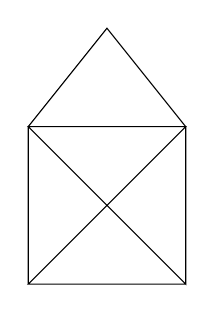
\begin{tikzpicture}
\draw (0,0) -- (0,2) -- (1,3.25) -- (2,2) -- (2,0) -- (0,2) -- (2,2) -- (0,0) -- (2,0);
\end{tikzpicture}
    
	\caption[Mit Tikz programmierte Grafik.]{Mit Tikz programmierte Grafik.}
	\label{fig:tikz_house}
\end{figure}

Ein etwas umfangreicheres Beispiel zur Digitaltechnik ist in Abbildung~\ref{fig:tikz_digital} dargestellt:

\begin{figure}[hbt]
	\centering
	\usetikzlibrary{circuits.logic.US,circuits.logic.IEC}
      \begin{tikzpicture}[circuit logic US]
      \matrix[column sep=7mm]
      {
      \node (i0) {0}; & & \\
      & \node [and gate] (a1) {}; & \\
      \node (i1) {0}; & & \node [or gate] (o) {};\\
      & \node [nand gate] (a2) {}; & \\
      \node (i2) {1}; & & \\
      };
      \draw (i0.east) -- ++(right:3mm) |- (a1.input 1);
      \draw (i1.east) -- ++(right:3mm) |- (a1.input 2);
      \draw (i1.east) -- ++(right:3mm) |- (a2.input 1);
      \draw (i2.east) -- ++(right:3mm) |- (a2.input 2);
      \draw (a1.output) -- ++(right:3mm) |- (o.input 1);
      \draw (a2.output) -- ++(right:3mm) |- (o.input 2);
      \draw (o.output) -- ++(right:3mm) node [right] {$y$ \quad Hier könnte Ihre Formel $y=(0 \land 0) \lor \overline{( 0 \land 1)}$ stehen};
 \end{tikzpicture}

	\caption[Mit Tikz programmierte Grafik, welche bereits vorgefertigte Bibliotheken für Symbole aus der Digitaltechnik nutzt.]{Mit Tikz programmierte Grafik, welche bereits vorgefertigte Bibliotheken für Symbole aus der Digitaltechnik nutzt.}
	\label{fig:tikz_digital}
\end{figure}

\clearpage

In der Tikz-Umgebung können auch Diagramme mit dem \textit{pgfplot}-Befehlssatz erzeugt werden. In Abbildung \ref{fig:pgfplot} sehen Sie ein Beispiel.

\begin{figure}[hbt]
	\centering
	\begin{tikzpicture}
		\begin{axis}[scale=1.3,legend entries={Messwerte mit Fehlerbalken,
			$\pgfmathprintnumber{\pgfplotstableregressiona} \cdot x  
			\pgfmathprintnumber[print sign]{\pgfplotstableregressionb}$}, legend style={draw=none},legend style={at={(0.01,0.98)},anchor=north west},xlabel=Stromstärke $I \; \mathrm{ \lbrack mA \rbrack}$,ylabel=Spannung $U \; \mathrm{ \lbrack V \rbrack}$]
		\addlegendimage{mark=*,blue}
		\addlegendimage{no markers,red}
\addplot+[error bars/.cd, y dir=both,y explicit]
table[x=x,y=y,y error=errory] 
{pgfplot/messdaten_mitfehler.dat};
\addplot table[mark=none,y={create col/linear regression={y=y}}]
{pgfplot/messdaten_mitfehler.dat};
	\end{axis}
\end{tikzpicture}
	\caption[Diagramm, erstellt mit dem \textit{pgfplot}-Befehlssatz.]{Ein Diagramm, erstellt in der \textit{tikzpicture}-Umgebung mit dem \textit{pgfplot}-Befehlssatz. Das Diagramm stellt Messdaten, deren Fehlerbalken und eine Regressionskurve dar. Die Messdaten werden von einer separaten Datei eingelesen und die Regressionskurve wurde mit \textit{pgfplot} berechnet und erstellt.}
	\label{fig:pgfplot}
\end{figure}

\clearpage

Auch hierzu der Quellcode in Listing~\ref{lst:pgfplot}.

\begin{lstlisting}[caption=Quellcode der Abbildung~\ref{fig:pgfplot}.,label=lst:pgfplot]
\begin{figure}[hbt]
\centering
\begin{tikzpicture}
		\begin{axis}[scale=1.3,legend entries={Messwerte mit Fehlerbalken,
			$\pgfmathprintnumber{\pgfplotstableregressiona} \cdot x  
			\pgfmathprintnumber[print sign]{\pgfplotstableregressionb}$}, legend style={draw=none},legend style={at={(0.01,0.98)},anchor=north west},xlabel=Stromstärke $I \; \mathrm{ \lbrack mA \rbrack}$,ylabel=Spannung $U \; \mathrm{ \lbrack V \rbrack}$]
		\addlegendimage{mark=*,blue}
		\addlegendimage{no markers,red}
\addplot+[error bars/.cd, y dir=both,y explicit]
table[x=x,y=y,y error=errory] 
{pgfplot/messdaten_mitfehler.dat};
\addplot table[mark=none,y={create col/linear regression={y=y}}]
{pgfplot/messdaten_mitfehler.dat};
	\end{axis}
\end{tikzpicture}
\caption[Diagramm, erstellt mit dem \textit{pgfplot}-Befehlssatz.]{Ein Diagramm, erstellt in der \textit{tikzpicture}-Umgebung mit dem \textit{pgfplot}-Befehlssatz. Das Diagramm stellt Messdaten, deren Fehlerbalken und eine Regressionskurve dar. Die Messdaten werden von einer separaten Datei eingelesen und die Regressionskurve wurde mit \textit{pgfplot} berechnet und erstellt.}
\label{fig:pgfplot}
\end{figure}
\end{lstlisting}

In Listing~\ref{lst:tikz} ist der Quellcode der Datei \textit{mess\_fehlerbalken.tex} dargestellt.

\begin{lstlisting}[caption=Quellcode der Datei \textit{mess\_fehlerbalken.tex}.,label=lst:tikz]
\begin{tikzpicture}
\begin{axis}[scale=1.3,legend entries={Messwerte mit Fehlerbalken,
$\pgfmathprintnumber{\pgfplotstableregressiona} \cdot x  
\pgfmathprintnumber[print sign]{\pgfplotstableregressionb}$}, legend style={draw=none},legend style={at={(0.01,0.98)},anchor=north west},xlabel=Stromstärke $I \; \mathrm{ \lbrack mA \rbrack}$,ylabel=Spannung $U \; \mathrm{ \lbrack V \rbrack}$]
\addlegendimage{mark=*,blue}
\addlegendimage{no markers,red}
\addplot+[error bars/.cd, y dir=both,y explicit]
table[x=x,y=y,y error=errory] 
{pgfplot/messdaten_mitfehler.dat};
\addplot table[mark=none,y={create col/linear regression={y=y}}]
{pgfplot/messdaten_mitfehler.dat};
\end{axis}
\end{tikzpicture}
\end{lstlisting}

\clearpage

In Abbildung~\ref{fig:pgfplot2y} wird ein weiters Beispiel für ein Diagramm gezeigt. Oftmals wird eine zweite y-Achse verwendet, um verschiedene Skalen darstellen zu können.

\begin{figure}[hbt]
	\centering
	\begin{tikzpicture}
%
\begin{axis}[
scale=1.3,
ytick pos=left,
xlabel=Zeit $t \; \mathrm{ \lbrack ns \rbrack}$,
ylabel=Spannung $U \; \mathrm{ \lbrack V \rbrack}$
]
\addplot[mark=*,only marks] table[x=x,y=y1] {pgfplot/messdaten_zweiyachsen.dat};
\end{axis}
%
\begin{axis}[
scale = 1.3,
legend style={draw=none},
legend style={at={(0.75,0.6)},
anchor=north west},
axis y line*=right,
axis x line=none,
%ymin=0,
%ymax=100,
ylabel=Strom $I \; \mathrm{ \lbrack mA \rbrack}$
]
\addlegendimage{mark=*,only marks}
\addlegendentry{Spannung}
\addplot[mark=x,only marks,blue] table[x=x,y=y2] {pgfplot/messdaten_zweiyachsen.dat};
\addlegendentry{Strom}
\end{axis}
\end{tikzpicture}
	\caption[Diagramm mit zwei unterschiedlichen y-Achsen.]{Diagramm mit zwei unterschiedlichen y-Achsen.}
	\label{fig:pgfplot2y}
\end{figure}

\clearpage

\subsection{Tabellen}

\begin{table}[hbt]	
	\centering
	\renewcommand{\arraystretch}{1.5}	% Skaliert die Zeilenhöhe der Tabelle
	\captionabove[Liste der verwendeten Messgeräte]{Liste der verwendeten Messgeräte. Die Genauigkeitsangaben beziehen sich auf die Standardabweichung $1\cdot \sigma$.}
	\label{tab:bsp}
	\begin{tabular}{ccccc}
		\textbf{Messgerät} & \textbf{Hersteller} & \textbf{Typ} & \textbf{Verwendung} & \textbf{Genauigkeit}\\ 
		\hline 
		\hline 
		\parbox[t]{0.2\linewidth}{\centering Spannungs-\\versorgung} & Voltmaker & HV2000 & \parbox[t]{0.2\linewidth}{\centering Spannungs-\\versorgung der\\Platine} & $\Delta U = \pm 5 $~mV \\ % Der parbox-Befehl ist erforderlich, damit ein Zeilenumbruch erzeugt werden kann. c-Spalten (zentriert) erlauben nicht automatisch einen Zeilenumpruch. Linksbündig gesetzte p-Spalten erlauben automatisch den Zeilenumbruch.
		Strommessgerät & Currentcount & Hotamp 16 & \parbox[t]{0.2\linewidth}{ \centering Strommessung\\am Versorgungspin\\des µC} & $\Delta I = \pm 0.1$~A \\ 
		\hline 
	\end{tabular} 
\end{table}

Der Quellcode der Beispieltabelle~\ref{tab:bsp} ist in Listing~\ref{lst:tab} zu sehen.

\begin{lstlisting}[caption=Quellcode der Tabelle~\ref{tab:bsp}.,label=lst:tab]
\begin{table}[hbt]	
\centering
\renewcommand{\arraystretch}{1.5}	% Skaliert die Zeilenhöhe der Tabelle
\captionabove[Liste der verwendeten Messgeräte]{Liste der verwendeten Messgeräte. Die Genauigkeitsangaben beziehen sich auf die Standardabweichung $1\cdot \sigma$.}
\label{tab:bsp}
\begin{tabular}{ccccc}
\textbf{Messgerät} & \textbf{Hersteller} & \textbf{Typ} & \textbf{Verwendung} & \textbf{Genauigkeit}\\ 
\hline 
\hline 
\parbox[t]{0.2\linewidth}{\centering Spannungs-\\versorgung} & Voltmaker & HV2000 & \parbox[t]{0.2\linewidth}{\centering Spannungs-\\versorgung der\\Platine} & $\Delta U = \pm 5 $~mV \\ % Der parbox-Befehl ist erforderlich, damit ein Zeilenumbruch erzeugt werden kann. c-Spalten (zentriert) erlauben nicht automatisch einen Zeilenumpruch. Linksbündig gesetzte p-Spalten erlauben automatisch den Zeilenumbruch.
Strommessgerät & Currentcount & Hotamp 16 & \parbox[t]{0.2\linewidth}{ \centering Strommessung\\ am Versorgungspin\\ des \textmu C} & $\Delta I = \pm 0.1$~A \\ 
\hline 
\end{tabular} 
\end{table}
\end{lstlisting}

\clearpage

\subsection{Formeln}

Formeln lassen sich in \LaTeX~ganz einfach schreiben. Es gibt unterschiedliche Umgebungen zum Schreiben von Formeln. Z.B. direkt im Text $v=s/t$ oder abgesetzt

\[F=m \cdot a\]

oder auch, wie in wissenschaftlichen Dokumenten üblich, nummeriert

\begin{equation}
P=\frac{U^2}{R} \quad .
\label{eqn:leistung}
\end{equation}

Mit einem Label in Formel~\ref{eqn:leistung} lassen sich natürlich auch Formeln im Text referenzieren. \LaTeX~verwendet im Formelmodus einen eigenen Schriftsatz, welcher entsprechend der gängigen Konventionen kursive Zeichen verwendet. Sollen im Formelmodus Einheiten in normaler Schriftart eingefügt werden, dann kann dies über den Befehl \textbackslash \textit{mathrm}\{\} erwirkt werden, wie im Quellcode von Formel~\ref{eqn:leistungMitEinh} zu sehen ist.

\begin{equation}
P=\frac{U^2}{R} = \frac{\left( 100~\mathrm{V}\right)^2}{100~\Omega} = 100~\mathrm{W}\quad .
\label{eqn:leistungMitEinh}
\end{equation}

Zum direkten Vergleich sind die Einheiten in Formel~\ref{eqn:leistungMitEinhfalsch} falsch dargestellt:

\begin{equation}
P=\frac{U^2}{R} = \frac{\left( 100~V\right)^2}{100\,\varOmega} = 100\,W
\label{eqn:leistungMitEinhfalsch}
\end{equation}

Zur einfachen Eingabe von Einheiten kann auch das Package \textbackslash \textit{siunitx} verwendet werden:

\begin{equation}
	P=\SI{100}{\watt}=\SI{100}{\joule\per\second}
\end{equation}

Das sind nur ein paar wenige Beispiele und es gibt sehr viele Packages, um Besonderheiten in Formeln realisieren zu können, z.B. mehrzeilige Formeln mit vertikaler Ausrichtung. Nennen Sie Formeln nur, wenn diese zum besseren Verständnis auch wirklich nützlich sind.

Folgende Befehle sind innerhalb von Formel-Umgebungen nützlich:
\begin{tabbing}
	\hspace*{0cm} \= \hspace{0.35\linewidth} \= \+\kill
	\textbackslash \textit{text}\{\}	\> Damit kann in Formel-Umgebung Text geschrieben werden.\\ 
	\textbackslash, \textbackslash: \textbackslash; oder \textbackslash quad und \textbackslash qquad \> Zusätzlichen Abstand zwischen Symbolen einfügen.\\
	\textbackslash \textit{notag} \> Nummerierung einer bestimmten Formel ausschalten.
\end{tabbing}

Abschließend nochmals ein kleines Beispiel:

\begin{eqnarray}
\sum\limits_{n=1}^\infty f\left(x_n\right)\cdot \Delta x=  \lim\limits_{\Delta x \rightarrow 0} \frac{f\left(x_0+\Delta x\right)-f\left(x_0\right)}{\Delta x} = \frac{\diff f}{\diff x} = \dot{f}(x)
\end{eqnarray}		% Zeile auskommentieren bei finalem Dokument!

\end{document}
